%%%% Pantalla(s) asociadas a caso de uso %%%%

\pagebreak
\hypertarget{IU1}{}
\section{IU1 Menú de Pizzas}

	%Descripción de la pantalla
	\noindent \textbf{Descripción de pantalla(s)}\\

		La pantalla mostrada en la figura \ref{IU1} tiene como objetivo permitir a los clientes mostrar el menú de pizzas que Pizza Planeta ofrece. 
		No se cuenta con campos de entrada. 
		
		El cliente podrá interactuar en la pantalla con los diferentes botones como se mostrará en la pantalla correspondiente a la figura \ref{IU1}.
		%Pantalla del sistema
		\begin{figure}[h]

			\begin{center}				

				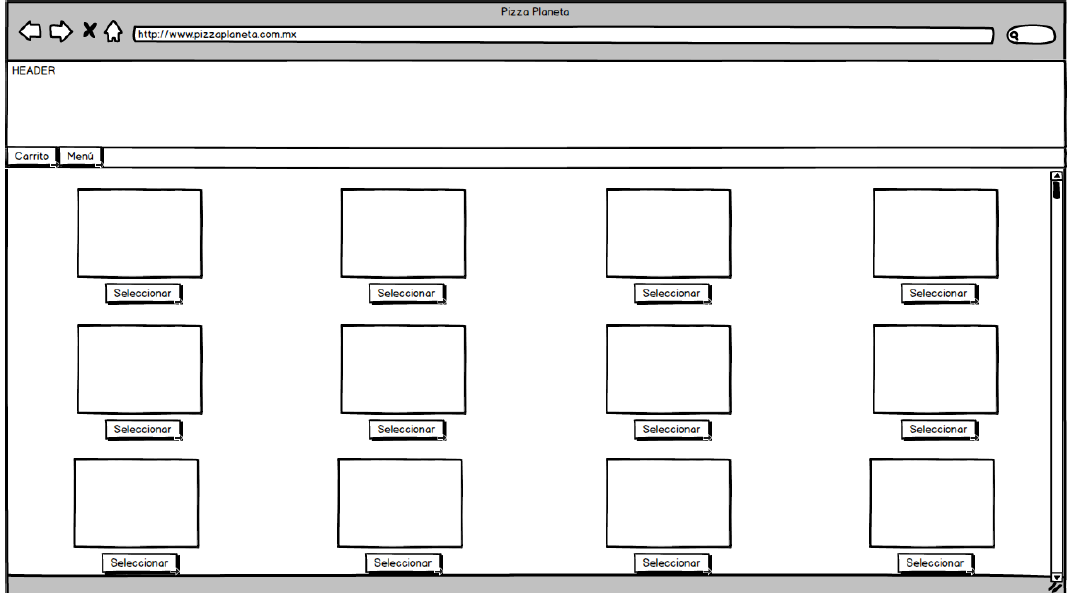
\includegraphics[scale=0.50]{./imagenes/IUs/RegistroSolicitantes/iu1-IniciarSesion/IU1-MenuDePizzas.png}
				\caption{IU1 Menú de Pizzas}
				\label{IU1}

			\end{center}
				
		\end{figure}


		El caso de uso \hyperlink{CU1}{CU1 Seleccionar Pizza}, describe de forma detallada el comportamiento asociado.

	%Acciones asociadas
	\noindent \textbf{\\Acciones en pantalla}

		\begin{itemize}

			\item 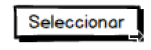
\includegraphics[scale=0.500]{imagenes/iconografia/Seleccionar.png}: Dirige a la pantalla \hyperlink{IU2}{IU2 Personaliza Pizza}
			\item 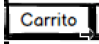
\includegraphics[scale=0.500]{imagenes/iconografia/Carrito.png}: Dirige a la pantalla \hyperlink{IU3}{IU3 Carrito de Compras}
			\item 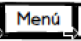
\includegraphics[scale=0.500]{imagenes/iconografia/Menu.png}: Dirige a la pantalla \ref{IU1}

		\end{itemize}


